% =========================================================================
% -------------------------------------------------------------------------
% Reactions: Chemical and Biological
% -------------------------------------------
%
%  This is a good place to outline key objectives of this section.
%
% -------------------------------------------------------------------------

\section{Biogeochemical Reaction Processes} 
\label{sec:biogeochemical}

A range of biogeochemical reaction processes may be included in the HPC Simulator, 
including multicomponent aqueous complexation, sorption (including simple linear distribution coefficient, or Kd, 
and more complex multicomponent and multisite surface complexation and ion exchange models), 
mineral dissolution and precipitation, and microbially-mediated reactions.  

% Spycher
\subsection{Aqueous Complexation} \label{sec:AqueousComplexation}

\subsubsection{Overview}

It is customary to treat the reaction network corresponding to the homogeneous reactions 
in the aqueous phase as a distinct set of processes taking place within a single aqueous phase \citep{steefel_1996}. 
%although these can also be described within the same more general formalism provided in Section~\ref{sec:mathframework} 
%that includes multiphase reactions.  
This reaction network is sometimes referred to as \textit{aqueous complexation}, 
since it involves reactions between individual dissolved species to form complexes.  

\subsubsection{Process Model Equations} \label{sec:aqueous-complexation-eq}

\paragraph{Equilibrium Reactions.} 

If we assume that the various aqueous species are in chemical
equilibrium, it is possible to reduce the number of
\textit{independent} concentrations, that is, the number that actually
need to be solved for. Mathematically, this means that in a system
containing $N_{tot} $ aqueous species, the number of independent
chemical components in the system $N_{c} $ is reduced from the total
number of species by the $N_{x} $ linearly independent chemical
reactions between them (for further discussion,
see~\citet{hooyman_1961, aris_1965, bowen_1968, van_1970, reed_1982,
  lichtner_1985, kirkner_1988}. This leads to a natural partitioning
of the system into $N_{c} $ \textit{primary} or \textit{basis}
species, designated here as $C_{j} $, and the $N_{x} $
\textit{secondary} species, referred to as $C_{i}
$~\citep{reed_1982, lichtner_1985, kirkner_1988}. The equilibrium
chemical reactions between the primary and secondary species take the
form
%
\begin{equation}
  \A_{i} 
     \rightleftharpoons 
        \sum _{j=1}^{N_{c} } \, 
        \nu _{ij} \A_{j} \; \; \; 
        (i=1,...,N_{x} ), 
\label{eq:AqueousComplexation:EquilibriumReaction} 
\end{equation} 
%
where $\A_{j} $ and $\A_{i} $ are the
chemical formulas of the primary and secondary species respectively
and $\nu _{ij} $ is the number of moles of primary
species $j$ in one mole of secondary species $i$. 
It should be noted here that the partitioning between the primary
and secondary species is not unique, that is, we can write the
chemical reactions in more than one way. The equilibrium reactions
provide an algebraic link between the primary and secondary species
via the law of mass action for each reaction
\begin{equation}
  C_{i} 
     = K_{i}^{-1} \gamma _{i}^{-1} 
       \prod _{j=1}^{N_{c} } \, 
          ( \gamma _{j} C_{j} )^{\nu _{ij}}
     \; \; \; 
     (i=1,...,N_{x} ), 
\label{eq:AqueousComplexation:MassAction} 
\end{equation} 
%
where $\gamma _{j} $ and $\gamma _{i} $ are
the activity coefficients for the primary and secondary species
respectively, and $K_{i} $ is the equilibrium
constant of the reaction given in
Equation~\eqref{eq:AqueousComplexation:MassAction}, written here as
the destruction\todo[color=cyan]{GEH: What does ``destruction'' mean?} of one mole of the secondary
species. Equation~\eqref{eq:AqueousComplexation:MassAction} implies
that the rate of production of a primary component $j$ due to
homogeneous reactions, $R_{j}^{aq}$, can be written in terms of the
sum of the total rates of production of the secondary
species~\citep{kirkner_1988}
%
\begin{equation}
  R_{j}^{aq} \eq -\sum _{i=1}^{N_{x} } \, \nu_{ ij} I_{i}^{aq} , 
 \label{eq:AqueousComplexation:RateSecondary} 
\end{equation} 
%
where $I_{i}^{aq}$ is the reaction rate of the secondary species in
the aqueous
phase. Equation~\eqref{eq:AqueousComplexation:RateSecondary} suggests
that one can think of a mineral dissolving, for example, as producing
\textit{only primary species} which then equilibrate instantly with
the secondary species in the system. Using
Equation~\eqref{eq:AqueousComplexation:RateSecondary} and neglecting
transport for the sake of simplicity here, the rates of the
equilibrium reactions can be eliminated~\citep{steefel_1996}
%
\begin{equation} \label{eq:PartitioningEquilibriumKinetic}
 \frac{\partial }{\partial t} \left[\phi s_w \rho _{w}  \left(C_{j} + \sum _{i=1}^{N_{x} } \, \nu _{ij} C_{i} \right)\right] =R_{j}^{min} \; \; \; (j=1,...,N_{c} ),
\end{equation} 
%\[
%\_ \boldsymbol{\nabla} \bullet \left[u\rho _{f} M_{H_{2} O} \left(C_{j} +\sum _{i=1}^{N_{x} } \, \nu _{ij} X_{i} \right)-D\boldsymbol{\nabla} \left\{\rho _{f} M_{H_{2} O} \left(C_{j} +\sum _{i=1}^{N_{x} } \, \nu _{ij} X_{i} \right)\right\}\right]
%\] 
%\begin{equation} \label{eq:AqueousComplexation:PrimaryTransport} 
%\_ =R_{j}^{min} \; \; \; (j=1,...,N_{c} ) 
%\end{equation} 
where $s_w$ and $\rho_w$ refer to the saturation and mass density of
the aqueous phase, respectively.  Note that only the term 
$R_{j}^{min} $ remains on the right hand side of
Equation~\eqref{eq:PartitioningEquilibriumKinetic} because we have
assumed that they are the only kinetic reactions.

\paragraph{Definition of a Total Concentration.}
\noindent If a total concentration, $\Psi_{j} $, is defined as~\citep{reed_1982, lichtner_1985, kirkner_1988} 
\begin{equation} \label{eq:AqueousComplexation_GrindEQ__12} 
  \Psi_{j} =C_{j} +\sum _{i=1}^{N_{x} } \, \nu _{ij} C_{i} , 
\end{equation} 
then the governing differential equations can be written in terms of the total concentrations in the case where only aqueous (and therefore mobile) species are involved (Kirkner and Reeves, 1988) 
\begin{equation} \label{eq:AqueousComplexation_GrindEQ__13} 
  \frac{\partial }{\partial t} \left( \phi s_w \rho _{w}  \Psi_{j} \right) 
  + 
  \boldsymbol{\nabla} \cdot \left[ \phi s_w \rho _{w} \boldsymbol{v}_w \Psi_{j} -D\boldsymbol{\nabla} 
  \left( \phi s_w \rho_{w}  \Psi_{j} \right) \right] \eq R_{j}^{min} \; \; \; (j=1,...,N_{c} ),
\end{equation} 
where $\boldsymbol{v}_w$ is the velocity of the aqueous phase and $R_j^{\rm min}$ denotes the kinetic mineral reaction rate.
As pointed out by~\citet{reed_1982} and~\citet{lichtner_1985}, the total concentrations can usually be interpreted in a straightforward fashion as the total elemental concentrations (e.g., total aluminum in solution), but in the case of $H^{+} $ and redox species, the total concentration has no simple physical meaning and the total concentrations may take on negative values. Such quantities, however, do appear occasionally in geochemistry, the best example of which is alkalinity. In fact, the alkalinity (which may take on negative values) is just the negative of the total H$^{+} $ concentration where CO$_{2}$(aq) or H$_{2}$ CO$_{3}$ is chosen as the basis species for the carbonate system. 

Note that the total concentration is generally only a useful concept computationally where equilibrium reactions allow the definition of secondary species described with Equation~\eqref{eq:AqueousComplexation:RateSecondary}.  In the case where the reactions among aqueous species are described kinetically, then the various aqueous complexes cannot be eliminated algebraically and they have to be solved for individually.

\paragraph{Kinetic Aqueous Reactions.}
If the aqueous phase reactions are not sufficiently fast for a given time scale of interest that they reach equilibrium, then they must be treated kinetically by solving an ordinary differential equation.  A convenient way to represent the reactions is with a Transition State Theory (TST) type of rate law~\citep{lasaga_1981, lasaga_1984, aagaard_1982}
\begin{equation} \label{eq:AqueousTSTkinetics}
  I_j^{aq} \eq k_{+}^{aq} \left(  \frac{Q^{aq}}{K^{aq}} \right) \prod a_{i}^{n},
\end{equation}
where $k_{+}^{aq}$ is the rate constant for the aqueous reaction, $Q^{aq}$ is the ion activity product , $K^{aq}$ is the corresponding equilibrium constant, and $a_i$ are the activities of the species affecting the rate far from equilibrium raised to the power $n$.

Alternatively, the reactions can be considered as completely irreversible, in which case there is no back reaction.  A good example is radioactive decay. The reactions are assumed to take the form
\begin{equation} \label{eq:IrreversibleKinetics}
  I_j^{aq} \eq k_{+}^{aq} \prod a_{i}^{n} ,
\end{equation}
and are therefore similar to the TST form except that a dependence on the saturation state is missing.   This more general form of irreversible reactions can be used to model decay and ingrowth of daughter products.

%\paragraph{References}

%\noindent Aagaard P. and Helgeson H.C. (1982) Thermodynamic and kinetic constraints on reaction rates among minerals and aqueous solutions, I, Theoretical considerations. \textit{Amer. J. Sci. }, 237-285. 
%
%\noindent Aris R. (1965) Prolegomena to the rational analysis of systems of chemical reactions. \textit{Arch. Rational Mech. and Anal.} , 81-99. 
%
%
%\noindent Bowen R.M. (1968) On the stoichiometry of chemically reacting materials. \textit{Arch. Rational Mech. Anal.} , 114-124. 
%
%
%\noindent Hooyman G.J. (1961) On thermodynamic coupling of chemical reactions. \textit{Proc. Nat. Acad. Sci.} , 1169-1173. 
%
%\noindent Kirkner D.J. and Reeves H. (1988) Multicomponent mass transport with homogeneous and heterogeneous chemical reactions: Effect of chemistry on the choice of numerical algorithm. I. Theory. \textit{Water Resources Res. }, 1719-1729. 
%
%\noindent Lasaga A.C. (1981) Rate laws in chemical reactions. In \textit{Kinetics of Geochemical Processes} (ed. A.C. Lasaga and R.J. Kirkpatrick), Rev. Mineral. , 135-169. 
%
%\noindent Lasaga A.C. (1984) Chemical kinetics of water-rock interactions. \textit{J. Geophys. Res. }, 4009-4025. 
%
%\noindent Lichtner P.C. (1985) Continuum model for simultaneous chemical reactions and mass transport in hydrothermal systems. \textit{Geochim. Cosmochim. Acta }, 779-800. 
%
%
%\noindent Reed M.H. (1982) Calculation of multicomponent chemical equilibria and reaction processes in systems involving minerals, gases, and an aqueous phase. \textit{Geochim. Cosmochim. Acta }, 513-528. 
%
%
%\noindent Steefel, C.I. and MacQuarrie, K.T.B. (1996) Approaches to modeling reactive transport in porous media.  In \textit{Reactive Transport in Porous Media} (P.C. Lichtner, C.I. Steefel, and E.H. Oelkers, eds.), \textit{Reviews in Mineralogy} 34, 83-125.
%
%
%
% 
%
%\noindent Van Zeggeren F. and Storey S.H. (1970) \textit{The Computation of Chemical Equilibria}. Cambridge University Press, Cambridge, 176 p. 
%
%


% Wolery
\subsection{Aqueous Activity Coefficients}   \label{sec:AqueousActivityCoefficients}

\subsubsection{Overview}

This Toolset
%~\todo{are we capitalizing toolset?  is toolset consistent with other documents? -Williamson} 
includes models for thermodynamic activity coefficients
in aqueous solutions. Multiple models, each with its own set of
parameters and limitations, will be provided. In general, the toolset
user must choose one such model to use in a given modeling
application. In setting up to run the application, the user must
ensure that a matching database with the requisite model-specific
parameters is provided to support the run.

A key solution parameter associated with aqueous species activity
coefficients is the ionic strength, defined as
\begin{equation}
  \label{eq:IonicStrength}
\bar{I} \eq \frac{1}{2} \sum _{i} m_{i} z_{i}^{2}.
\end{equation}
Here $m_{i}$ denotes the molal concentration (molality) of the
$i^{th}$ solute species and $z_{i}$ denotes its electrical charge
number. Activity coefficients of charged solute species include a
functional dependence on the ionic strength. The exact nature of this
dependence depends on the specific model.

Activity coefficient models can be classified as to the upper limit of
ionic strength to which a given model provides generally satisfactory
results. For the most part, there are two kinds of such models. Low
ionic strength models are generally usable up to an ionic strength of
more or less 1 molal. Examples include the Davies equation and the
B-dot equation. These models are based on simple equations and have a
relatively small number of associated parameters. High ionic strength
models are usable to very high ionic strength ($>$20 molal).
The highest
values of ionic strength normally seen are limited by the solubilities
of highly soluble salts, such as calcium chloride and calcium nitrate.
Examples of high ionic strength models include Pitzer's equations and
Extended UNIQUAC. High ionic strength models have more complex
equations and require substantially more parameters than low ionic
strength models. They are most likely to be applied to problems in
which the ionic strength is higher than 1 molal. At low ionic
strength, it is generally preferable to use a low ionic strength
model, because the number of required parameters is smaller. In many
instances, there will be sufficient supporting data available to
support the use of low ionic strength models for large numbers of
chemical components and species, but that may not be the case for the
high ionic strength models. There are activity coefficient models that
extend to intermediate ionic strength (4-6 molal). The NEA SIT
model is an example. These models tend to be intermediate in equation
complexity and number of required parameters. They have not received
much attention to date in modeling geochemically complex systems.

It is noted that low ionic strength models are sufficient for many EM
applications. Hanford tanks and the WIPP site pose notable exceptions, requiring the
use of high ionic strength models. There may be other instances in
which the use of low ionic strength models may be inappropriate. 

There are two kinds of activity coefficients that a model should be
able to provide. The first is the molal activity coefficient of a
solute species (denoted by $\gamma _{i}$). This is subsequently used
to compute the thermodynamic activity of the corresponding species
(denoted by $a_{i}$). The activity of a species is obtained by
multiplying the molality (molal concentration) of the species (denoted
by $m_{i}$) by the molal activity coefficient:
%
\begin{equation}
  a_{i} =m_{i} \gamma _{i}.
\end{equation}
%
This activity is then used in various equations describing
thermodynamic equilibrium and chemical kinetics. 

The second kind of activity coefficient, the rational activity
coefficient, pertains to the solvent, water ($w$). Its activity
coefficient is denoted by $\lambda_{w}$ to emphasize that it is
different in kind: it is a mole fraction activity coefficient. The
thermodynamic activity of water ($a_{w}$) is obtained by multiplying
the mole fraction of water ($X_{w}$) by the activity coefficient of
water:
\begin{equation}
a_{w} \eq X_{w} \lambda _{w} .
\end{equation}
The activity of water is also different in kind from the activity of a
solute species (a mole fraction activity as opposed to a molal
activity).  In treating the thermodynamics of aqueous electrolyte solutions,
the activity of water and the activity of a solute species are almost
always treated as described above.

\todo[color=cyan]{GEH: Why are we including this discussion of log vs ln?}Activity coefficients are generally first calculated in logarithmic
form (e.g., $\ln \gamma_{i}$ or $\log \gamma_{i}$). In practical
usage, activity coefficients are used most often used in base-10
logarithmic form, being converted from natural logarithm form as
necessary. The conversion is illustrated by
\begin{equation}
\log\gamma_{i} =\frac{\ln\gamma_{i}}{\ln (10)}.
\end{equation}
The conversion factor $\ln(10)$ is approximately equal to 2.303, and
this value often appears in equations in the literature in place of
the exact factor. The approximate value should not be used in this
toolset, as it is insufficiently precise for accurate work. Instead
the value should be calculated using the same floating-point precision
that will be used to calculate activity coefficients. This is most
efficiently done by calculating the value once and then storing it for
subsequent use. 
It is noted that ``log'' is somewhat ambiguous, in
that the literature contains examples of it being used for both
natural and base-10 logarithms. In the present description given in this section (Section~\ref{sec:AqueousActivityCoefficients}), 
it will always refer to the base-10 logarithm.

Activity coefficient model equations ideally satisfy thermodynamic
consistency relations. The value of consistency lies in allowing the
possibility of accuracy at higher ionic strengths. Low ionic strength
models typically include inconsistent equations, but the numerical
consequences of the inconsistencies tend to be acceptable in the range
of applicability of these models. For electrolyte solutions,
\citet{wolery-1990} presents equations and methods for ensuring the
development of 
consistent equations and for testing the consistency of existing sets
of equations. The easiest means of testing for consistency is to use
the cross-differentiation rule, which takes the following forms for
solute-solute and solvent-solute pairs:
\begin{eqnarray}
\frac{\partial\ln\gamma_{j}}{\partial m_{i}} &=&\frac{\partial\ln\gamma_{i}}{\partial m_{j}}, \\
N_{w}^{kg} \, \frac{\partial \ln a_{w}}{\partial m_{i} } &=&-1-\sum _{j}m_{j} \frac{\partial \ln \gamma_{i}}{\partial m_{j}}
\end{eqnarray}
where $i$ and $j$ denote different solute
species and $N_{w}^{kg}$ is the number of moles of water in a 1 kg mass
(approximately 55.51).

\subsubsection{The Debye-H\"{u}ckel Equations} 
\label{sec:debyehuckel}

Activity coefficient model equations for electrolyte solutions
generally include some type of Debye-H\"{u}ckel term to represent the
effects of long-range electrical forces. The most common
representation is based on the ``extended'' Debye-H\"{u}ckel equation,
which for the activity coefficient of an ionic solute species is given
by
%
\begin{equation}
   \log \gamma _{i} = - A_{\gamma ,10} z_{i}^{2} 
                       \left( \frac{\sqrt{ \bar{I} }}{1 + b \sqrt{\bar{I}}} \right).
\end{equation}
%
Here $A_{\gamma ,10} $ is the Debye-H\"{u}ckel ``$A$'' parameter for the
activity coefficient (hence the subscript ``$\gamma$''), modified for
consistency with the base-10 \todo[color=cyan]{GEH: I suggest that we pick one convection for log (base-10) vs. natural log and stick with it throughtout this entire document.}logarithmic activity coefficient on the
left-hand-side of the equation (hence the additional subscript,
``10''). To assist in avoiding potential confusion, $A_{\gamma ,10}$
should have a value of 0.5114 at
25${}^\circ$C and 1.013 bar pressure. The parameter ``$b$'' is
conceptually the product of the Debye-H\"{u}ckel ``$B$'' parameter for
the activity coefficient ($B_{\gamma}$) and a length that
corresponds to either the diameter of the ion in question or a
characteristic distance of closest approach to itself or any other ion
in solution. Practical models treat this in various ways. Some assign
a constant value, typically 1.0, 1.2, or 1.5. Others use the product
of $B_{\gamma}$ (which has a known temperature and pressure
dependence) and some sort of length parameter.

The equation for the activity of water corresponding to the extended
Debye-H\"{u}ckel equation is
%
\begin{equation}  \label{eq:ActivityWater}
  \log a_{w} = \frac{1}{N_{w}^{kg} } 
                 \left( - \frac{\sum _{i}m_{i}}{\ln(10)} 
                        + \frac{2}{3} A_{\gamma ,10} \bar{I}^{3/2}
                          \varsigma(b\sqrt{\bar{I}})
                 \right).
\end{equation}
%
where the summation over molalities spans all solute
species (all aqueous species except the solvent), and the function
$\varsigma $(x) in Equation~\eqref{eq:ActivityWater} is given by
\begin{equation}
  \varsigma (x) \eq \frac{3}{x^{3} } \left(1+x-\frac{1}{1+x} -2\ln (1+x)\right),
\end{equation}
where $x$ serves the purpose of a generic variable.
If the activity coefficient of water is desired, it can be obtained
from the relation
%
\begin{equation}
   \log \lambda _{w} \eq \log a_{w} -\log (X_{w} ),
\end{equation}
%
where the mole fraction of water is given by
%
\begin{equation}
   X_{w} \eq \frac{N_{w}^{kg} }{N_{w}^{kg} +\sum _{i}m_{i}  } .
\end{equation}
%
The activity of water is closely related to the osmotic coefficient, $\varphi$:
%
\begin{equation}
   \varphi \eq -\left(\frac{N_{w}^{kg} }{\sum _{i}m_{i}  } \right)\ln a_{w} .
\end{equation}

All forms of the extended Debye-H\"{u}ckel equation are consistent with
the Debye-H\"{u}ckel Limiting Law (DHLL):
%
\begin{equation}
   \lim \limits_{\bar{I}\to 0} \log \gamma _{i} \eq -A_{\gamma ,10} z_{i}^{2} \sqrt{\bar{I}}.
\end{equation}
%
The limiting law is a critical feature describing the behavior of
ionic activity coefficients in the range of very low ionic strength.
The ionic activity coefficient plunges rapidly from unity as ionic
strength increases from zero. There is no comparable limiting relation
for the activity of water, due to the compositional dependence on both
the ionic strength and the sum of solute molalities.

In general, the extended Debye-H\"{u}ckel equation is not useful for
significant practical modeling, as it is accurate only in very dilute aqueous
solutions. If only monovalent ions are present, it may be useful for
$\bar{I} < $ 0.1 molal. In the presence of higher valence ions, the
maximum range becomes more compressed. Most practical models therefore
extend the ``extended'' Debye-H\"{u}ckel equation by adding additional
terms or otherwise adding to the mathematical complexity, in the
process introducing more model parameters.

The activity coefficient models that will be available in this toolset
include the Davies equation, the B-dot equation, Pitzer's equations,
Extended UNIQUAC, and NEA-SIT. The models are first addressed, followed by  
the discussion on rescaling the activity coefficients.

\subsubsection{The Davies Equation} 
\label{sec:davies}

The \citet{CWDavies_1962} equation is a commonly used at low ionic strength (less
than about 1 molal) model. The activity coefficient of an aqueous
solute species is given by
%
\begin{equation}
  \log \gamma _{i} \eq - A_{\gamma ,10} z_{i}^{2} 
                      \left( \frac{ \sqrt{ \bar{I} } }{1 + \sqrt{ \bar{I} } }- d \bar{I}  \right).
\end{equation}
%
Here $d$ is a constant, either 0.2 as in EQ3/6 \citep{Wolery-1992}
or 0.3 as in PHREEQC (Parkhurst and Appelo, 1999). If the
``$d \bar{I}$'' part is dropped, this equation reduces to the extended
Debye-H\"{u}ckel form with $b$ set to unity. It can be shown
that the full equation satisfies the solute-solute-form of the
cross-differentiation rule.

For the activity coefficient of water, the matching equation used in
EQ3/6 for the activity of water is
\begin{equation}
  \log a_{w} \eq \frac{1}{N_{w}^{kg} } \left(-\frac{\sum _{i}m_{i}  }{\ln (10)} 
  +
  \frac{2}{3} A_{\gamma ,10} \bar{I}^{\frac{3}{2} } \varsigma (\sqrt{\bar{I}} )-dA_{\gamma ,10} \bar{I}^{2} \right).
\end{equation}
where all parameters and the $\varsigma (x)$ function have been
previously introduced (See Section~\ref{sec:debyehuckel}). This
equation is a corrected version of that given by \citet{Wolery-1992}
(Equation 86 in that document). Here a factor of 2 in the 
``\textit{d}'' term has been
removed, and $d$ substitutes for the original constant value of
0.2. This equation is quasi-consistent with the equation for the
activity coefficient of a solution species, in the sense that the
solvent-solute form of the cross-differentiation rule is satisfied for
the case of a pure solution of a uni-univalent electrolyte, such as
sodium chloride. It does not satisfy this rule in the general case.

The equation used by PHREEQC is symbolically equivalent to
\begin{equation}
  a_{w} \eq 1 - \frac{1}{N_{w}^{kg} } \sum _{i}m_{i}.  
\end{equation}
As given by the source (Parkhurst and Appelo, 1999, p. 17), the
factor 1/$N_{w}^{kg} $ is replaced by a constant value of 0.017, which is
rather approximate, and the molality is replaced by the mole number
divided by the number of kg of solvent water (this substitution is
exact). This equation is based on ignoring the activity coefficient of
water and replacing the mole fraction with a limiting approximation of
itself. Hence, the activity of water is given in direct form, rather
than logarithmically.

For the present toolset, it is recommended that the Davies model be
implemented as two options, one (Davies-EQ3/6) consistent with the
implementation in EQ3/6, the other (Davies-PHREEQC), with
PHREEQC. This will permit direct comparison with both codes.

The Davies equation predicts a unit activity coefficient for
electrically neutral solute species. This is known to be generally
inaccurate, as the activity coefficients of non-polar neutral solutes
such as O$_2$(aq) and N$_2$(aq) should increase with ionic strength (the
``salting out'' effect), while the activity coefficients of polar
species such as CaSO$_4$(aq) and MgSO$_4$(aq) should decrease
(``salting-in'').

In practice, the Davies equation is mainly used for low temperatures
(near 25${}^\circ$C) and near-atmospheric pressures. The $A_{\gamma
,10}$ parameter has temperature and pressure dependence. As long as
this is accounted for, the Davies equation model could be applied in
principle at higher temperatures and pressures. However, it needs to
be kept in mind that the 0.2 constant was obtained by fitting data to
solutions for temperature near 25${}^\circ$C and for atmospheric
pressure. The accuracy of the model is therefore likely to deteriorate
at higher temperatures and pressures.

\subsubsection{The B-dot Equation} 
\label{sec:b_dotEquation}

The B-dot equation of \citet{helgeson-1969} is an alternative low ionic
strength model. The activity coefficient of a solute species is given
by
%
\begin{equation}
   \log \gamma _{i}  
      \eq - \frac{A_{\gamma ,10} z_{i}^{2} \sqrt{ \bar{I} }}
               {1+ \mathring{a_i} B_{\gamma } \sqrt{\bar{I}}} 
        + \dot{B} \bar{I}.
\end{equation}
%
where $\mathring{a_i}$ is the diameter of the $i^{th}$ solute species,
$B_{\gamma } $ is the Debye-H\"{u}ckel B parameter for the activity
coefficient, and $\dot{B}$ is the ``B-dot'' parameter.  Removing the
$\dot{B}\bar{I}$ term and setting $\mathring{a} B_{\gamma }$ to unity, this
equation reduces to the Davies equation with the $d\bar{I}$ term omitted.
Comparison with the Davies equation brings up two points. The first is
that the B-dot model has more parameters.  The $B_{\gamma}$ parameter
appears, and each solute species has an assigned diameter. The
``B-dot'' parameter itself is an additional parameter.

It can be shown that the B-dot equation does not satisfy the
solute-solute form of the cross-differentiation rule. There is an
issue with the first term on the right hand side in that the rule can
only be satisfied if all aqueous ions have the same diameter. There is
an issue with the second term in that the rule is only satisfied if
the charge number squared is the same for all ions, as would be the
case for example in a pure sodium chloride solution.

For an electrically neutral species, the B-dot equation reduces to
%
\begin{equation}
  \log \gamma _{i} \eq \dot{B}\bar{I}.
\end{equation}
%
As the $\dot{B}$ parameter is generally assigned a positive value, this
would provide for some measure of ``salting-out.'' By tradition,
however, the B-dot equation is not applied to neutral solute species,
and it will not be so applied in the present toolset. For non-polar
neutral species, the common practice is to assign an approximation for
the activity coefficient of CO$_2$(aq) in otherwise pure sodium chloride
solution of the same ionic strength. The approximation used in EQ3/6
(based on \citet{drummond-1981}, and which will be adopted for the present
toolset) is
%
\begin{equation}
  \ln \gamma_{i} \eq \left( C + FT + \frac{G}{T} \right) I 
                  -( E + HT ) \left( \frac{\bar{I}}{\bar{I} + 1} \right).
\end{equation}
%
Here T is the absolute temperature and C = -1.0312, F = 0.0012806, G =
255.9, E = 0.4445, and H = -0.001606. Note that the result is
presented in terms of the natural logarithm.
For a polar aqueous species, the EQ3/6 practice (which will be adopted
in the present toolset) is to use
%
\begin{equation}
\log \gamma _{i} \eq 0.
\end{equation}
%
Because different equations are used for electrically neutral solute
species than for ionic species, there is necessarily an additional set
of violations of the solute-solute cross-differentiation rule.

For the activity of water, the B-dot model as implemented in EQ3/6
(and recommended for the present toolset) is to use the equation
%
\begin{equation}
   \log a_{w} 
   = \frac{1}{N_{w}^{kg}} 
     \left( - \frac{\sum _{i}m_{i}}{\ln (10)} 
            + \frac{2}{3} A_{\gamma ,10} \bar{I}^{\frac{3}{2}} 
              \sigma( {\mathring{a}} B_{\gamma} \sqrt{\bar{I}} )
            - \dot{B}\bar{I}^{2} 
     \right).
\end{equation}
%
All the parameters here have been introduced previously, except for
the unsubscripted $\mathring{a}$, which is conceptually an effective solute species
diameter. In practice, this is assigned a constant value of 4.0
angstroms.

The above equation for the activity of water is quasi-consistent with
the solvent-solute form of the cross-differentiation rule. The term
containing the effective solute diameter leads to inconsistency unless
every ionic solute has a matching diameter value. The term containing
$\dot{B}$ leads to inconsistency unless the solution is a pure
solution of a uni-univalent electrolyte such as sodium chloride.

The thermodynamic inconsistencies noted above introduce some level of
inaccuracy into the model, tending to negate the improvement that
might be expected by introducing more parameters (e.g., a diameter
value specific to each solute species). Thus, for temperature near
25${}^\circ$C and near-atmospheric pressure, the B-dot model is
probably as good as the Davies equation model.

The B-dot model does have an advantage over the Davies equation model
in that it is better parameterized to cover a wide range of
temperature and pressure. In addition to $A_{\gamma ,10}$, the
$B_{\gamma} $and $\dot{B}$ parameters are treated as functions of
temperature and pressure. The $A_{\gamma ,10} $ and $B_{\gamma}$ 
parameters have values derived from pure theory (and models for pure
water properties). The $\dot{B}$ parameter is obtained by fitting to
data for pure sodium chloride solutions. The ion size parameters are
treated as constant with respect to temperature and pressure.

In regard to solute species, diameters are only necessary for ionic
species. Some means needs to be provided to specify (as on a
supporting thermodynamic data file) whether a neutral species is to be
treated as non-polar or polar. All the necessary information could be
folded into a diameter array or equivalent structure, in which the
values in the case of neutral species would not be actual diameters,
but code values specifying non-polar or polar type. However, a
separate flagging structure should be utilized, as the variable type
can then be something more appropriate (integer or logical) than the
floating point necessary for actual diameters. Also, the structure for
diameters would then be free to include diameters for neutral solute
species. Although such diameters are not be used in the B-dot model,
they might be usable in other models.

\include{Pitzer}

\include{UNIQUAC}

\include{NEA-SIT}

\subsubsection{Rescaling Ionic Activity Coefficients}

The activity coefficient models described above include descriptions
of individual ion activity coefficients. This is problematic in that
ionic activity coefficients and ionic activities are not measurable
for individual ions. These quantities are measurable only in
combinations that correspond to electrical neutrality. For activity
coefficients, examples of such combinations include 
$\log \gamma_{H^{+} } +\log \gamma_{Cl^{-} }$ and 
$2\log \gamma_{H^{+} } +\log \gamma_{SO_{4}^{2-}}$; 
examples for activities are analogous.
Molalities of individual ions are measureable (or quantifiable by
inference). Thus, if one could obtain or specify the activity or
activity coefficient of one single ion in an aqueous solution, one
could then use this as a reference to obtain the activities and
activity coefficients of all other ions present in the same solution.

The need to define activity coefficients and activities for individual
ionic species is dealt with by the use of a ``splitting'' convention.
Such a convention is at least somewhat arbitrary, although it may be
guided in part by theoretical concerns. One could address the issue by
adopting the results of model equations for single ion activity
coefficients. The model equations for these are all in part arbitrary,
implicitly including a splitting based on some combination of
theoretical notions and pleasing (but not necessarily unique)
symmetry. The problem with just using the model equations in their
native form is that other conventions have been previously adopted
into measurement practice, particularly the measurement of pH. For
accurate modeling consistent with standard analytical chemistry
practice, it becomes necessary to rescale the results of the model
equations presented above. This only affects the activity coefficients
of ionic species. For most analytical splitting conventions, some
expression is specified for the activity coefficient of a reference
ion, usually Cl$^-$ or H$^+$.

The most significant analytical splitting conventions for aqueous ions
are tied to the definition of the pH. Conceptually,
%
\begin{equation}
   pH = -\log a_{H^{+}} .
\end{equation}
%
In order to provide a practical basis for measuring the pH, it is
necessary to define the activity of the hydrogen ion. The splitting
convention used for this purpose then defines a pH scale. The choice
of pH scale further affects the definition of the redox potential, E$_h$. %\todo{subscript h? - Williamson}

In modern work, the dominant pH scale is the NBS scale, originated by
the National Bureau of Standards, now the National Institute of
Standards and Technology. The NBS scale is based on the
Bates-Guggenhiem equation \citep{bates-1964}:
%
\begin{equation}
  \log \gamma _{Cl^{-} } =-\frac{A_{\gamma ,10} \sqrt{\bar{I}}}{1+1.5\sqrt{\bar{I} } } .
\end{equation}
%
This is a simple form of the extended Debye-H\"{u}ckel equation. It
defines the activity coefficient of the chloride ion. It may be
surprising that chloride is used as the reference ion rather than the
hydrogen ion, which is more closely tied to the pH.  What is apparent is that the Bates-Guggenheim
equation must give a result that is different from what would be
obtained for the chloride ion using say the Davies equation or the
B-dot equation, or for that matter, from Pitzer's equations. In the
range of low ionic strength (say less than 1 molal), the differences
should be numerically small for each of the three practical models, as
they and the Bates-Guggenheim equation all include some form of
extended Debye-H\"{u}ckel model and thus are all consistent with the
Debye-H\"{u}ckel limiting law.  At higher ionic strength, however, the differences can be substantial (the equivalent of several pH units). 

The Bates-Guggenheim equation can be applied whether or not there is
any chloride in aqueous solution, as the equation is sufficient to
calculate the specified activity coefficient. The charge number of -1
is effectively built into the equation. 

The Bates-Guggenheim equation (the NBS pH scale) is effectively built
in to the calibration of all modern means of measuring the pH, whether
in pH calibration buffers or pH paper. EQ3/6 for example by default
rescales ionic activity coefficients computed from the models to be
consistent with the NBS pH scale (other options, including no
rescaling, may be offered). Rescaling from one scale (scale ``1'') to
another (scale ``2'') is accomplished using 
%
\begin{equation}
   \log \gamma_{i}^{(2)} 
     = \log \gamma_{i}^{(1)} 
     + \frac{z_{i}}{z_{j}} 
       \left( 
         \log \gamma_{j}^{(2)} - \log \gamma_{j}^{(1)} 
       \right).
\end{equation}
%
Here $j$ denotes the reference ion (here Cl$^-$) and $i$ denotes any ion
(including the reference ion). In the present context, scale ``1'' is
usually that implied by a model equation and scale ``2'' is the
desired scale.

An alternative convention is to choose
%
\begin{equation}
  \log \gamma _{H^{+}} = 0.
\end{equation}
%
For the hydrogen ion, this results in
% 
\begin{equation}
  pH = -\log m_{H^{+}} .
\end{equation}
%
as the activity and molality of the hydrogen ion are numerically
equivalent. The rescaling of ionic activity coefficients for
consistency does not give an analogous result for other ions. EQ3/6
allows rescaling using this convention as an option, but it has
limited utility and it not recommended as a general option in the
present toolset.

The definition of the pH in terms of molality (``pmH'') is significant independent of rescaling. Thus one has simply

\begin{equation}
  pmH = -\log m_{H^{+} } .
\end{equation}
%
In concentrated electrolyte solutions (e.g., WIPP, Hanford tanks), pmH
is often more useful for assessing the acidity/basicity of a solution
than the NBS pH. The NBS pH cannot be accurately measured in
concentrated solutions owing to liquid junction effects with
electrodes and interferences with dyes. Also, the Bates-Guggenheim
equation (and the NBS pH scale itself) was originally intended for use
only at low ionic strength. \citet{bates-1964} suggested application
to solutions with ionic strengths of no greater than 0.1 molal. Since
then, however, the scale has been used at higher ionic strengths. This
has led to the problem that of two highly concentrated solutions with
an NBS pH of say 2, one might be acidic (in the sense that H+ is
abundant) and the other not (in the sense that H+ is not abundant). In
other words, the common association of pH values with various degrees
of acidity/basicity (e.g., 7 is neutral) no longer applies.

Still other conventions and scales exist. However, for the present
toolset only the following is required. First, the default behavior
will be to apply rescaling to the NBS scale. Second, the option will
be available to use the basic model results without rescaling. Third,
the pmH will be directly calculated and included in the output. An
option to rescale the activity coefficients for consistency with the
$\log \gamma _{H^{+}} = 0$ convention will not be required.

 


% Liange
% Tell Texshop where the project root is
%!TEX root = requirements.tex
%
\subsection{Sorption}  \label{sec:Sorption}

\subsubsection{Overview} 

Sorption involves the attachment of dissolved and/or colloidal species to mineral or other solid surfaces.  Sorption has the effect of slowing the effective transport rate of a species through porous media through its retardation effect.  The retardation effect for a species, $R_f$, is given by~\citep{bouwer-1991}
\begin{equation}
  R_f = \frac{V_{gw}}{V_{sp}},
\end{equation}
where 
$V_{gw}$ is the velocity of the groundwater and $V_{sp}$ is the velocity of the species.  
A variety of models have been used to describe sorption and can be broadly divided 
into those that describe it as a bulk process versus those that are mineral or solid phase specific.  
The latter approach involves the calculation of  bulk sorption from the sum of sorption on individual solid phases, 
an assumption referred to as \textit{Component Additivity}.  
Within the class of bulk sorption models, a distinction can be made between those 
which assume a finite number of sorption sites (these are referred to as showing 
Langmuir type behavior and include the Langmuir isotherm itself and most surface complexation 
and ion exchange models) and those that assume either an infinite sorption capacity 
or at least a capacity that is not tightly constrained 
(these include the linear distribution coefficient and the nonlinear Freundlich isotherm).  
Alternatively, one could also distinguish between single component, 
non-competitive models (e.g., Langmuir and Freundlich) and multicomponent competitive models (surface complexation and ion exchange).

Another possible distinction is between equilibrium and kinetic sorption models.  
In many cases, the formulations for the equilibrium and kinetic cases differ 
only insofar as the kinetic case involves involves a thermodynamic driving force 
(as in the equilibrium case), but modified by a finite rate constant.  
In some cases, however, sorption is described as irreversible, which implies that there is no back reaction (desorption).

%%\paragraph{Assumptions, Approximations, Applicability.}


\subsubsection{Process Model Equations}

\paragraph{Linear Distribution Coefficients ($K_d$).}
A simple approach to describe metal or ionic radionuclide sorption by a sediment,
\begin{equation}
  A_{aq}\leftrightharpoons A_{ads},
\end{equation}
is to use a constant distribution coefficient, defined by:
\begin{equation} \label{eq:Kd} 
  K_d = \frac{[A_{ads}]}{[A_{aq}]},
\end{equation} 
where $K_d$ is the distribution coefficient (L/kg), $[A_{ads}]$ is the sorbed concentration (mol/kg) to the bulk solid phase, 
and $[A_{aq}]$ is the total dissolved concentration in groundwater (mol/L) \citep{davis-1990}.  
One of the key advantages of representing sorption with a distribution coefficient is that it can be easily incorporated 
into reactive transport models used for migration predictions. 

Equation \eqref{eq:Kd} shows that if one assumes that the amount of sorption is proportional to the dissolved concentration, 
then there is a linear relationship where the $K_d$ value is the slope. 
In this simple case, referred to as a linear isotherm, retardation of a concentration  front in simple porous media is given by
%
\begin{equation}  \label{eq:KdRetardation}
  \frac{\bar{v}}{\bar{v}_{c} } 
  =
  1+\frac{\rho _{b} }{n} K_{d}  ,
\end{equation}
where $\rho_b$ is the bulk density, 
$n$ the porosity, 
$\bar{v}$ the average linear velocity of the groundwater and 
$\bar{v}_{c} $ the velocity of the point on the concentration profile 
where the concentration is half that of the input concentration \citep{freeze-1979}. 
Note that the ratio $\bar{v}$/$\bar{v}_{c} $ here is the retardation factor and represents 
the retardation of the movement of front relative to the flowing groundwater. 
While this is a simplified example, it serves to illustrate the key point that the $K_d$ value 
directly influences predictions of adsorbing metal or radionuclide mobility. 

%Could have the following
\subparagraph{Assumptions and Applicability} 
Sorption is proportional to the dissolved concentration. 
The aqueous and adsorbed phases are in equilibrium.

\subparagraph{Data Needs}
Typically $K_d$ values are determined for a particular subsurface material 
from the slope of a fitted line to the concentration of the sorbed species, $A_{ads}$, 
plotted versus the dissolved concentration of the same species, $A_{aq}$.  
These data may be derived from laboratory analyses, where one typically varies the dissolved concentrations systematically, 
or they may be derived from in situ field data.  
Since $K_d$ values may be variable, and in particular a function of temperature, 
pH or the redox state of the system (see below), it is often necessary to compile them in a lookup table for use by a particular computer code.

\paragraph{Langmuir Isotherm.}
The Langmuir isotherm assumes that the sorption sites, S, on the surface of a solid (absorbent) become occupied 
by an absorbate from the solution, A.  Implying a 1:1 stoichiometry
%
\begin{equation}  \label{eq:langmuir} 
  S + A \leftrightharpoons SA,
\end{equation}
where $SA$ is the adsorbed species on the surface. At equilibrium, a
standard mass action equation can be written:
%
\begin{equation}  \label{eq:langmuir_massaction}
  K_{ads,L} = \frac{ [ SA ] }{ [S] \{A\} },
\end{equation}
where the square brackets here refer to the concentration of the
species or site, and the curly brackets refer to the aqueous
activity.  Using the maximum concentration of surface sites, $S_T$
%
\begin{equation}  \label{eq:totalsurfacesites}
  [S_T] = [S] + [SA],
\end{equation}
one can write the Langmuir isotherm in its familiar hyperbolic form
%
\begin{equation}  \label{eq:hyperbolicLangmuir}
  [SA] = [S_T] \frac{ K_{ads} \{A\} }{1 + K_{ads} \{A\} }.
\end{equation}

%Could have the following
\subparagraph{Assumptions} 
For the following, it is assumed that the surface and aqueous species are in equilibrium.

\subparagraph{Data Needs} 
The equilbrium constant, $K_{ads}$, is typically obtained from experimental data. 
It depends on the specified absorbent and absorbate, and may be a function of temperature. 
It may be calculated from:
\begin{equation}
  K_{ads} = \exp\left(\frac{-\Delta G^{\circ}_{ads}}{RT}\right),
\end{equation}
where $\Delta G$ is the change in free energy for the reaction,
typically obtained from a database, $R$ is the gas constant and $T$ is the temperature.

\paragraph{Freundlich.} 
The Freundlich isotherm is another equilibrium model for sorption of absorabte A onto sorption sites, S
\begin{equation}  \label{eq:langmuir_reaction} 
  S + A \leftrightharpoons SA.
\end{equation}
Represented by the mass action equation:
\begin{equation}
  K_{ads,F} = \frac{ [ SA ] }{ \{A\}^{\beta_F} },
\end{equation}
where the square brackets again refer to the concentration of the
species or site, the curly brackets refer to the aqueous activity.
$K_{ads,F}$ and ${\beta_F}$ are the Freundlich parameters
\citep[e.g.][]{langmuir-1997, stumm-1992}.

%Could have the following
\subparagraph{Assumptions} 
For the following, it is assumed that the surface and aqueous species are in equilibrium.

\subparagraph{Data Needs} 
The Freundlich parameters, $K_{ads,F}$ and $n$, are generally obtained by fits to experimental data 
for a specific surface and aqueous species. 
They will generally be obtained from a database, and 
may be represented by a functional form or lookup table.

%Steefel
\paragraph{Multi-site, Multi-component Ion Exchange.}
An ion exchange reaction can be described via a mass action expression
with an associated equilibrium constant \citep{vanselow-1932,sposito-1981,appelo-1993}.  
The exchange reaction can be written in generic form as
\begin{equation}
  vACl_{u} (aq)+uBX_{\nu } (s)\leftrightharpoons uBCl_{\nu } (aq)+vAX_{u} (s),
\end{equation} 
where X refers to the exchange site occupied by the cations $A^{u+}$ and $B^{v+}$.  
The equilibrium constant, $K_{eq}$, for this reaction can be written as \citep{vanselow-1932}
\begin{equation}
  K_{eq} =\frac{\{BCl_{\nu } \}^{u} \{AX_{u}\}^{\nu } }{\{ACl_{u} \}^{\nu } \{BX_{\nu } \}^{u} },
\end{equation} 
where the curly braces refer to the thermodynamic activities.
Several activity conventions are in wide use.  One possibility is the
Gaines-Thomas activity convention, which assumes a reaction
stoichiometry of the following form \citep{appelo-1993}, written
here assuming the $Cs^+$ is the relevant cation of interest
\begin{equation}
  Cs^{+} + (1/z) MX(i)_{z} \leftrightharpoons CsX(i) + (1/z) M^{z+},
\end{equation} 
where $M$ is the competing cation ($Na^+$, $K^+$, $Ca^{++}$), $z$ is
its charge, and $X(i)$ refers to the $i^{th}$ type of exchange site.  
In the Gaines-Thomas convention, each exchange site, $X(i)$ has a charge of -1. 
The activities of adsorbed species correspond to the charge equivalent fractions, $\beta (i)_{M} $,
\begin{equation}
  \beta (i)_{M} =\frac{z_{M} q(i)_{M} }{\sum _{M}z_{M} q(i)_{M}  } = \{X(i)_{M} \},
\end{equation} 
where $z_M$ is the charge of cation $M$, $q(i)_M$ is the concentration
of adsorbed cation $M$ in exchange site \textit{i} (moles/g),
and the curly brackets denote activities.  
The Gapon activity convention is obtained by writing the reactions in every case with a
single exchanger \citep{appelo-1993}.  
Alternatively, the Vanselow convention \citep{vanselow-1932} describes the exchanger activity
with mole fractions
\begin{equation}
  \beta (i)_{M} =\frac{q(i)_{M} }{\sum _{M}q(i)_{M}  } = \{ X(i)_{M} \}.
\end{equation} 
The exchange reactions can then be used to write a mass action equation for binary Cs-M exchange:
\begin{eqnarray}
  K_{M/Cs} & = & \frac{\beta (i)_{M} ^{1/z} \{Cs^{+} \}}{\beta (i)_{Cs} \{M^{z+} \}^{1/z} } \\
  & = & 
\frac{\{X(i)_{M} \}^{1/z} \{Cs^{+} \}}{\{X(i)_{Cs} \}\{M^{z+} \}^{1/z} } .
\end{eqnarray}

In a single-site ion exchange model, the CEC is equal to the sum of the charge equivalent concentrations of the adsorbed cations:
\begin{equation}
  CEC = \sum _{M}z_{M} q_{M},
\end{equation} 
while in a multi-site model, the CEC is the charge summed over all of the cation exchange sites \citep{cernik-1996, voegelin-2000}
\begin{equation}
  CEC = \sum _{i}\sum _{M}z_{M} q(i)_{M}   .
\end{equation} 

%Could have the following
\subparagraph{Assumptions} 
For the following, it is assumed that the surface and aqueous species are in equilibrium.
%\todo{Need short description here}

%%\subparagraph{Data Needs}
%%\todo{Need short description here}

\paragraph{Surface Complexation.} 
\label{sec:surfaceComplexation} An alternative approach that allows a modeler to describe sorption while
simultaneously considering variable chemical conditions in the subsurface is a surface complexation model \citep{davis-2004}.  
In this approach, the sorbing sediment surfaces are considered to possess
surface functional groups that can form complexes analogous to the
formation of aqueous complexes in solution.  
These surface reactions include proton exchange, cation binding and anion binding via ligand
exchange at surface hydroxil sites (represented here as $XOH$ to avoid
confusion with other chemical species). 
For example, the sorption of a metal could be represented as
%
\begin{equation} \label{eq:metalSorption} 
  XOH + M^{z_+} \leftrightharpoons XOM^{z_+ - 1} + H^{+}  .
\end{equation} 

At equilibrium, the sorption reactions can be described by the mass law equation
%
\begin{equation} \label{eq:sorptionMassAction}
  K_{app} =\frac{\left[XOM^{z_{+}-1 } \right]\{H^{+} \} }{\left[XOH\right] \{M^{z+} \} }  ,
\end{equation} 
where $K_{app}$ is referred to as the apparent equilibrium constant,
because it includes surface charge effects and hence is dependent on
the extent of surface ionization \citep{dzombak-1990}, $\{i\}$
is the thermodynamic activity of aqueous species $i$, and the terms in
square brackets represent the concentration of surface complexes (mol/kg).

Surface complexation differs from the simpler isotherm and
ion-exchange models in several important ways. Surface complexation is
based on the electrical double layer (EDL) theory. EDL theory assumes
that the surface charge of a sorbent in contact with solution
generates an electrostatic potential that declines rapidly away from
the sorbent surface, creating an electrostatic field. An additional
energetic term accounting for the work needed for the aqueous species
to travel across the surface electric field is required:
%
\begin{eqnarray} \label{eq:EDLdeltaG}
\Delta G_{ads} & = & \Delta G_{intr} + \Delta G_{coul} \nonumber \\
               & = & \Delta G_{intr} + (\Delta G_{\psi =0} - \Delta G_{\psi =\psi_{0} } ) \nonumber \\
               & = & \Delta G_{intr} - z F \psi_{0}  .
\end{eqnarray} 
\noindent where $\Delta G_{ads} $ is the free energy change of the overall adsorption reaction, $\Delta G_{intr} $ and $\Delta G_{coul} $ are the free energy change due to chemical bonding and to the electrostatic work (Coulombic attraction), respectively, $z$ is the charge of the surface species, $F$ the Faraday's constant (96485 C/mol), and $\psi _{0} $ is the mean surface potential ($V$). Since
%
\begin{equation} \label{eq:deltaGKeq}
  \Delta G = -RTlnK,
\end{equation}
%
\noindent Equation~\eqref{eq:EDLdeltaG} can be rewritten as
\begin{equation} \label{eq:KappEDL} 
K_{app}  = K_{int} \exp\left({\frac{z F \psi _{0} }{RT} } \right),
\end{equation} 
where $R$ is the gas constant (8.314 J/mol/K), $T$ is the absolute
temperature (K), and $K_{int}$ is the intrinsic equilibrium constant
which does not depend on the surface charge.

%Could have the following
%\subparagraph{Assumptions}
%\subparagraph{Issues Associated with the Application of Surface Complexation}

\subparagraph{Bulk and Mineral Specific Surface Complexation. }

There are two major approaches for applying the surface complexation
concept to soils and sediments: the Component Additivity (CA) and
Generalized Composite (GC) approaches \citep{davis-2004, davis-1998}. In
the CA approach, it is assumed that a mineral assemblage is composed
of a mixture of one or more reference phases, whose surface chemical
reactions are known from independent studies of each phase \citep[e.g.][]{
landry-2009, davis-2004, arnold-2001}. Based
on a measurement of the relative amounts or surface areas of each
mineral present in the soil or sediment, sorption by the mixture of
phases can be predicted by an equilibrium calculation, without any
fitting of experimental data for the mixture. CA model predictions are
sometimes made by assuming that one mineral component dominates
sorption \citep{zhang-2009, davis-2004, payne-2004, barnett-2002},
% Barnett et al., 2002
allowing a straightforward equilibrium calculation, if the exposed
surface area of that mineral component in the soil or sediment can be
quantified.

In the GC approach, the surface of the mineral assemblage is
considered too complex to be quantified in terms of the contributions
of individual phases to sorption and/or that the contribution of
individual components is not additive. The complexity is caused, in
part, by the difficulties in quantifying the electrical field and
proportions of surface functional groups at the mineral-water
interface in the mixture of mineral phases and associated surface
coatings. In the GC approach, it is assumed that sorption can be
described by mass laws written with ``generic'' surface functional
groups, with the stoichiometry and formation constants for each mass
law determined by fitting experimental data for the mineral assemblage
as a whole \citep{hyun-2009, bond-2008, davis-2004}. 
%Bond et al., 2008;
The GC modeling approach has generally been applied using a
non-electrostatic model (NEM), which considers surface equilibria
strictly as chemical reactions without explicit correction for
electrostatic attraction or repulsion \citep{yabusaki-2008,
  davis-2004, kent-2000}. In an NEM, the apparent binding constants
and stoichiometry of the mass action equations are derived by fitting
the \textit{macroscopic} dependence of adsorption as a function of pH
\citep{davis-1998}. Because of the exclusion of electrical double
layer terms, the mass action equations are not expected to provide
accurate representations of the stoichiometry of the reactions
\textit{at the molecular scale}, however, the surface reactions can
still be coupled with aqueous complexation reactions to provide
simulations of macroscopic sorption as a function of aqueous chemical
conditions.

Although there are differences between the GC and CA approaches, 
they are very similar with respect to their scientific basis. 
The following concepts form the basic tenets of both GC and CA modelling approaches \citep{davis-1998}:

\begin{enumerate}
\item Mineral surfaces are composed of chemical functional groups that can react with dissolved solutes to form surface complexes (coordinated
%~\todo{coordinated? - Williamson} 
complexes or ion pairs) in a manner analogous to aqueous complexation reactions in homogeneous solutions.

\item The equilibria of surface complexation and ionization reactions can be described via mass law equations, either with or without correction factors applied for electrostatic attraction to or repulsion from the surface.

\item The apparent binding constants determined for the mass law equations of surface complexation and ionization reactions are semi-empirical parameters related to thermodynamic constants via rational activity coefficients for surface species.
\end{enumerate}

Both CA and GC models may: 
\begin{enumerate}
\item be coupled to the same critically reviewed aqueous thermodynamic data
\item use spectroscopic data to constrain and/or determine surface complex chemical composition and stoichiometry, and 
\item use the same mass laws and surface species. 
\end{enumerate}
The differences among the model approaches lie primarily in the manner in which the models are calibrated and assumptions about various model parameters (in particular, whether the contributions of the various mineral phases to sorption and electrostatic fields can be considered as additive). CA models have almost always been applied using mass laws with electrostatic correction factors, while GC models have not usually used these factors.

\subparagraph{Experimental and Modeling Issues Associated with SCMs for Soils and Sediments.}

Common to all applications of surface complexation approaches in soils
and sediments is an initial characterization with respect to surface
area, bulk mineralogy, and clay and organic carbon content.  In
addition, if the sediment is already contaminated with a metal or
radionuclide, a measurement of the labile fraction of the contaminant
needs to be determined \citep{kohler-2004, curtis-2004, bond-2008}.

In the GC approach, laboratory experiments are conducted with the field site sediments across the range of chemical conditions that are relevant to the scenarios of the physical and temporal modeling domains. Then, mass law relationships are derived that describe the change in metal or radionuclide sorption with variations in the aqueous chemical conditions \citep{davis-2004}.  Total surface functional groups are typically estimated from surface area measurements.  The number of surface site types and surface binding reactions is a practical modeling decision made based on the goodness-of-fit and the desired number of modeling parameters \citep{hyun-2009}.

In the CA modeling approach, after the sediment mineralogy is known, an estimate of the distribution of mineral surface areas is made.  This can be done by simply assuming that the bulk weight abundances of various mineral phases are related to the distribution of functional groups at the sediment surface.  For example, if quartz represents 60\% by weight of the sediment, then an initial estimate could be that 60\% of the surface area is represented by the quartz surfaces. Then a model of metal or radionuclide adsorption on quartz (as a function of chemical conditions relevant to the field site) is chosen from available literature data.  Similar models for other minerals in the sediment are also catalogued.  In some cases, model parameters may need to be re-derived from the original experimental data to develop a dataset that is self-consistent. In particular, this may be necessary if different electrical double layer models were used in the reference mineral models.  Other approaches for estimating the distribution of mineral surface areas may be used, including chemical extractions and other methods \citep{davis-2004, davis-1998}.  Once the component mineral models have been chosen, a predictive calculation of metal or radionuclide sorption for a specific set of chemical conditions can be made.

Possible limitations inherent to the surface complexation approach include poor representation of: a) surface functional groups, b) surface area, c) electrical double layer properties, d) surface species, e) surface binding constants, and f) competing surface reactions and their electrostatic effects. These limitations exist for both GC and CA modeling approaches, but the GC approach attempts to resolve some of the issues by using empirical data to overcome unknown factors and unmeasured parameters. For example, consider the representation of surface functional groups: Assume that only silanol, aluminol, ferrinol, and clay mineral edge sites are of importance in a particular sediment sample. At present it is very difficult or expensive to determine the distribution of mineral surface areas in a mixed mineral assemblage. Extractions, X-ray diffraction, and surface spectroscopies have been used by various investigators, but each of these methods provides estimates that are difficult to confirm independently. This uncertainty is circumvented in the GC approach by assuming that the distribution of site types is an unknowable quantity, and only generic sites are used. However, this requires that experimental data for the metal or radionuclide sorption on a site-specific sediment sample are collected, whereas in principle at least, additional characterization experiments are not needed for the CA modeling approach.

\subparagraph{Quantifying Surface Sites}

Surface area is an important experimental quantity to be characterized in all surface complexation approaches. Typically a mixed mineral assemblage is characterized by BET analysis of nitrogen gas adsorption. Adjustments may need to be made for samples that contain high abundances of clay minerals, depending on whether there is evidence of sorption on the basal planes of clay mineral particles. Many investigators have concluded that surface functional groups of the basal planes are unreactive for metal and radionuclide sorption, and therefore the surface area of the basal planes does not need to be included in most applications. Fortunately, the BET method does not typically measure the surface area of the basal planes. In GC applications, the surface area is typically used in a straightforward manner to quantify the total abundance of surface sites using a conversion factor. In CA applications, however, the surface area should be distributed among different functional group types.

Multiple site-types are commonly used in formulating SCMs and approximate the nonlinear isotherms commonly observed for cation adsorption on well-characterized oxide mineral phases \citep{dzombak-1990, davis-1990}.  Postulating multiple site-types is also important for simulating peak tailing observed in experimental studies of U(VI) transport in columns \citep{kohler-1996}.  Reactive transport simulations that use multisite adsorption models can also simulate significant peak tailing in field-scale simulations \citep{curtis-2006, kent-2000, kent-2007, kent-2008}. 

%\subparagraph{Data Needs}

\subparagraph{Sub-models}

\begin{enumerate}
\item \textbf{Non-electrostatic Models:}
EDL models differ in whether coulombic attraction or repulsion terms are considered in the mass laws of surface reactions. A non-electrostatic EDL means that the term
\begin{equation}  \label{eq:ElectrostaticExponential}
  \exp\left(\frac{zF\psi_0 }{RT}\right) 
\end{equation}
in Equation~\eqref{eq:KappEDL} need not be considered. 
While electrical double layer (EDL) models may represent these terms well for simple systems with single mineral phases, 
the approaches for treating these terms in mixed mineral assemblages have not been studied. 
In Component Additivity (CA) \citep{davis-2004, davis-1998} applications to sediments, 
typically authors assume that the EDL properties of pure, clean mineral phases 
investigated remain the same in mixed mineral assemblages \citep{davis-2004}. 
This ignores the likely effects of surface contaminants (adsorbed major solutes such as silicate, organic compounds, etc.) 
and the overlapping EDL regions of particles that are known to change coulombic terms. 
In Generalized Composite (GC) approaches \citep{davis-2004, davis-1998}, 
the coulombic attraction or repulsion terms are not included, 
but are instead built into the semi-empirical model calibration of reaction stoichiometries and binding constants to experimental data. 
That is, whatever EDL forces exist, they are lumped into the model fitting of reactions and binding constants. 
In each case, there is inherent uncertainty in the modeling approach. 
The errors within the GC model may not be that significant because of model calibration to experimental data, 
but the error is only minimized by confining model calculations to chemical conditions interpolated between those 
investigated in laboratory experiments. 
Extrapolation of any non-electrostatic model to uninvestigated chemical conditions is unwise 
because the EDL forces for those conditions will not necessarily be captured accurately by the model calibration. 
In addition the formation of unknown surface species may not be realized if calculations are extrapolated to chemical conditions 
not investigated at all.

\item \textbf{Electrostatic models:}
When the coulombic attraction or repulsion terms is considered as shown in Equation~\eqref{eq:KappEDL}, 
the electrostatic models differs also among themselves in how they conceptualize the structure of the double-layer 
and describe changes in surface potential and surface charge from the surface of the sorbent phase to the bulk solution. 
In the constant capacity and diffuse-layer models, all adsorbed species are considered specifically adsorbed at the zero plane 
while the triple layer model can assign adsorbed species to either a zero plane or more distant plane. 
The constant capacity and diffuse-layer model are elaborated in the following sections.  

\begin{enumerate}
\item \textbf{Constant Capacitance} The constant capacitance model is
  a special case of the diffuse-layer model. Both models are based on
  the assumption that all the species are adsorbed in the same layer
  and a diffuse layer of counterions constitutes the transition to
  homogenous solution.  Additionally, it is assumed that the surface
  potentials are small, or the double layer has been compressed (very
  high ionic strength).  However, differently from the diffuse-layer
  model, the relationship between the surface charge and the potential
  is assumed to be linear:
%
\begin{equation} \label{eq:constantCapacitance} 
  \sigma  = \mathbb{C}\psi  ,
\end{equation} 
where $\sigma$ is the surface charge, $C\;m^{-2}$, $\psi$ is the
potential at the surface, $V$, and $\mathbb{C}$ is a constant
capacitance value, $C\;V^{-1}\;m^{-2}$, to be obtained from fitting
experimental data.  Equation~\eqref{eq:constantCapacitance} is solved
for the potential and substituted into Equation~\eqref{eq:KappEDL}.

\item \textbf{Diffuse Double Layer Model}
The diffuse layer model has been described in great detail by \citet{dzombak-1990} and was applied to adsorption of metals on iron oxide surfaces. In the diffuse layer model, the solid-water interface is composed of two layers: a layer of surface-bound complexes and a diffuse layer of counter ions in solution. The surface charge is calculated from the total surface species adsorbed on the layer:
\begin{equation} \label{eq:doubleLayerSurfaceChargeDensity} 
  \sigma _{p} = \frac{F}{A} \sum _{k=1}^{N_{s} } z_{k} y_{k}  .
\end{equation} 
Here $A$ is the surface area sorbent per liter solution ($m^2/L$), $F$ is the
Faraday constant ($96,480 C/mol$), $z_k$ is the charge of the ion, and $y_k$ is the concentration (mol/L) of surface bound ions in the Stern Layer.  According to the Gouy-Chapman theory, the surface charge density $\sigma_{p}$ ($C/m^2$) is related to the potential at the surface (volts) by:
\begin{equation} \label{eq:doubleLayerGouyChapman} 
  \sigma _{p}  =  (8RT\epsilon_R \ \epsilon _{0}\; C_e \times 10^{3} )^{1/2} \sinh \left(\frac{zF \psi _0 }{ 2RT}\right)  ,
\end{equation} 
where $R$ is the molar gas constant (8.314 $J mol^{-1} K^{-1}$), $C_e$
is the molar electrolyte concentration ($M$), $z$ is the electrolyte
charge, $T$ is the absolute temperature ($K$), $\epsilon_R$ is the
relative dielectric constant of water ($\epsilon = 78.5$ at
$25^{\circ}C$), and $\epsilon_{0}$ is the permittivity of free space
($8.854\times 10^{-12}$ $C\;V^{-1} m^{-1}$).  Equation
\eqref{eq:doubleLayerGouyChapman} is only valid for a symmetrical
electrolyte, the anion and cation must have the same charge.  Note
that $C$ the unit (coulombs or celcius) is not a concentration.
Capacitance is not solved for explicitly, but is implicitly accounted
for in Equation~\eqref{eq:doubleLayerGouyChapman}.  It is common to use
the linearized version of Equation \eqref{eq:doubleLayerGouyChapman} for
low values of the potential:
%
\begin{equation} \label{eq:doubleLayerLinearizedGouyChapman} 
  \sigma _{p} =\epsilon \ \epsilon _{0} \kappa \psi _{0},
\end{equation} 
where $1/\kappa$ (m) is the double-layer thickness defined as
%
\begin{equation} \label{eq:doubleLayerThickness} 
  \frac{1}{\kappa }  = \left( \frac{\epsilon \ \epsilon_{0} RT}{2 F^{2} \cdot 1000 \;I} \right)^{1/2}  ,
\end{equation} 
where $I$ is the ionic strength $mol\;L^{-1}$. The first term of Equation~\eqref{eq:doubleLayerGouyChapman}, $(8RT\epsilon \ \epsilon _{0} C_e \times 10^{3} )^{1/2}$, can be rewritten at $25^{\circ}C$:
%
\begin{equation} \label{eq:doubleLayerGouyChapman25} 
  \mathop{\sigma }\nolimits_{p} = 0.1174\;C_e^{1/2} \sinh \left( \frac{zF \psi_d}{2RT} \right) .
\end{equation} 
Therefore, in the diffuse-layer model, the value of the capacitance $\mathbb{C}$ relating the surface charge and the potential can be calculated based on theoretical considerations instead of being an experimental fitting parameter.

\item \textbf{Triple Layer Model} 
The triple layer model is similar to the double layer model, but
divides the sorbed species into two layers,
Figure~\ref{fig:triple-layer-model}. Strongly sorbed species are
located close to the surface, the zero plane, while weakly sorbed
species reside in the beta plane, seperated from the surface by the
strongly sorbed species and hydration layers \citep[e.g.][]{langmuir-1997}. Further out from the surface is a diffuse layer and the bulk solution similar to the double
layer.

The charge balance equation for the triple layer model is
\begin{equation}
  \sigma_0 + \sigma_{\beta} + \sigma_d = 0,
\end{equation}
\noindent where $\sigma_0$, $\sigma_{\beta}$ and $\sigma_d$ are the
net surface charges in the zero, beta and diffuse planes respectively, ($C/m^2$).
The net surface charge in the zero plane is given by:
\begin{equation}    \label{eq:ChargeDensityZeroPlane}
  \sigma_0 =  \frac{F}{A} \sum _{k=1}^{N_{s} } z_{k} y^{0}_{k}  ,
\end{equation}
where the variables are as defined in Equation \eqref{eq:doubleLayerSurfaceChargeDensity} with the exception of $y^{0}_{k}$, which is the concentration (mol/L) bound in the zero plane. Similarly, the net surface charge of the beta plane is
\begin{equation}    \label{eq:ChargeDensityBetaPlane}
  \sigma_{\beta} =  \frac{F}{A} \sum _{k=1}^{N_{s} } z_{k} y^{\beta}_{k}  ,
\end{equation}
where $y^{\beta}_{k}$ refers to the ions bound in the beta plane.
Note that the composition of the diffuse layer is not often calculated explicitly in either Triple Layer Model or the Diffuse Double Layer Model, although a method to do so has been presented by \citet{leroy2007modeling}.

The triple layer model assumes constant capacitances between the zero
plane and beta plane, $\mathbb{C}_1$, and the beta plane and d-plane, $\mathbb{C}_2$.
These are related to the surface charges and potentials by:
%\todo{Two captions here and it is not referenced. -Williamson}
\begin{eqnarray}
  \sigma_0 &=& \mathbb{C}_1 \left( \psi_0 - \psi_{\beta} \right), \\
  \sigma_{\beta} &=& \mathbb{C}_1 \left( \psi_{\beta} - \psi_0 \right) + \mathbb{C}_2 \left( \psi_{\beta} - \psi_d \right),\\
  \sigma_{d} &=& \hspace{28mm}\mathbb{C}_2 \left( \psi_d - \psi_{\beta} \right).
\end{eqnarray}

\begin{figure}
  \begin{center}
    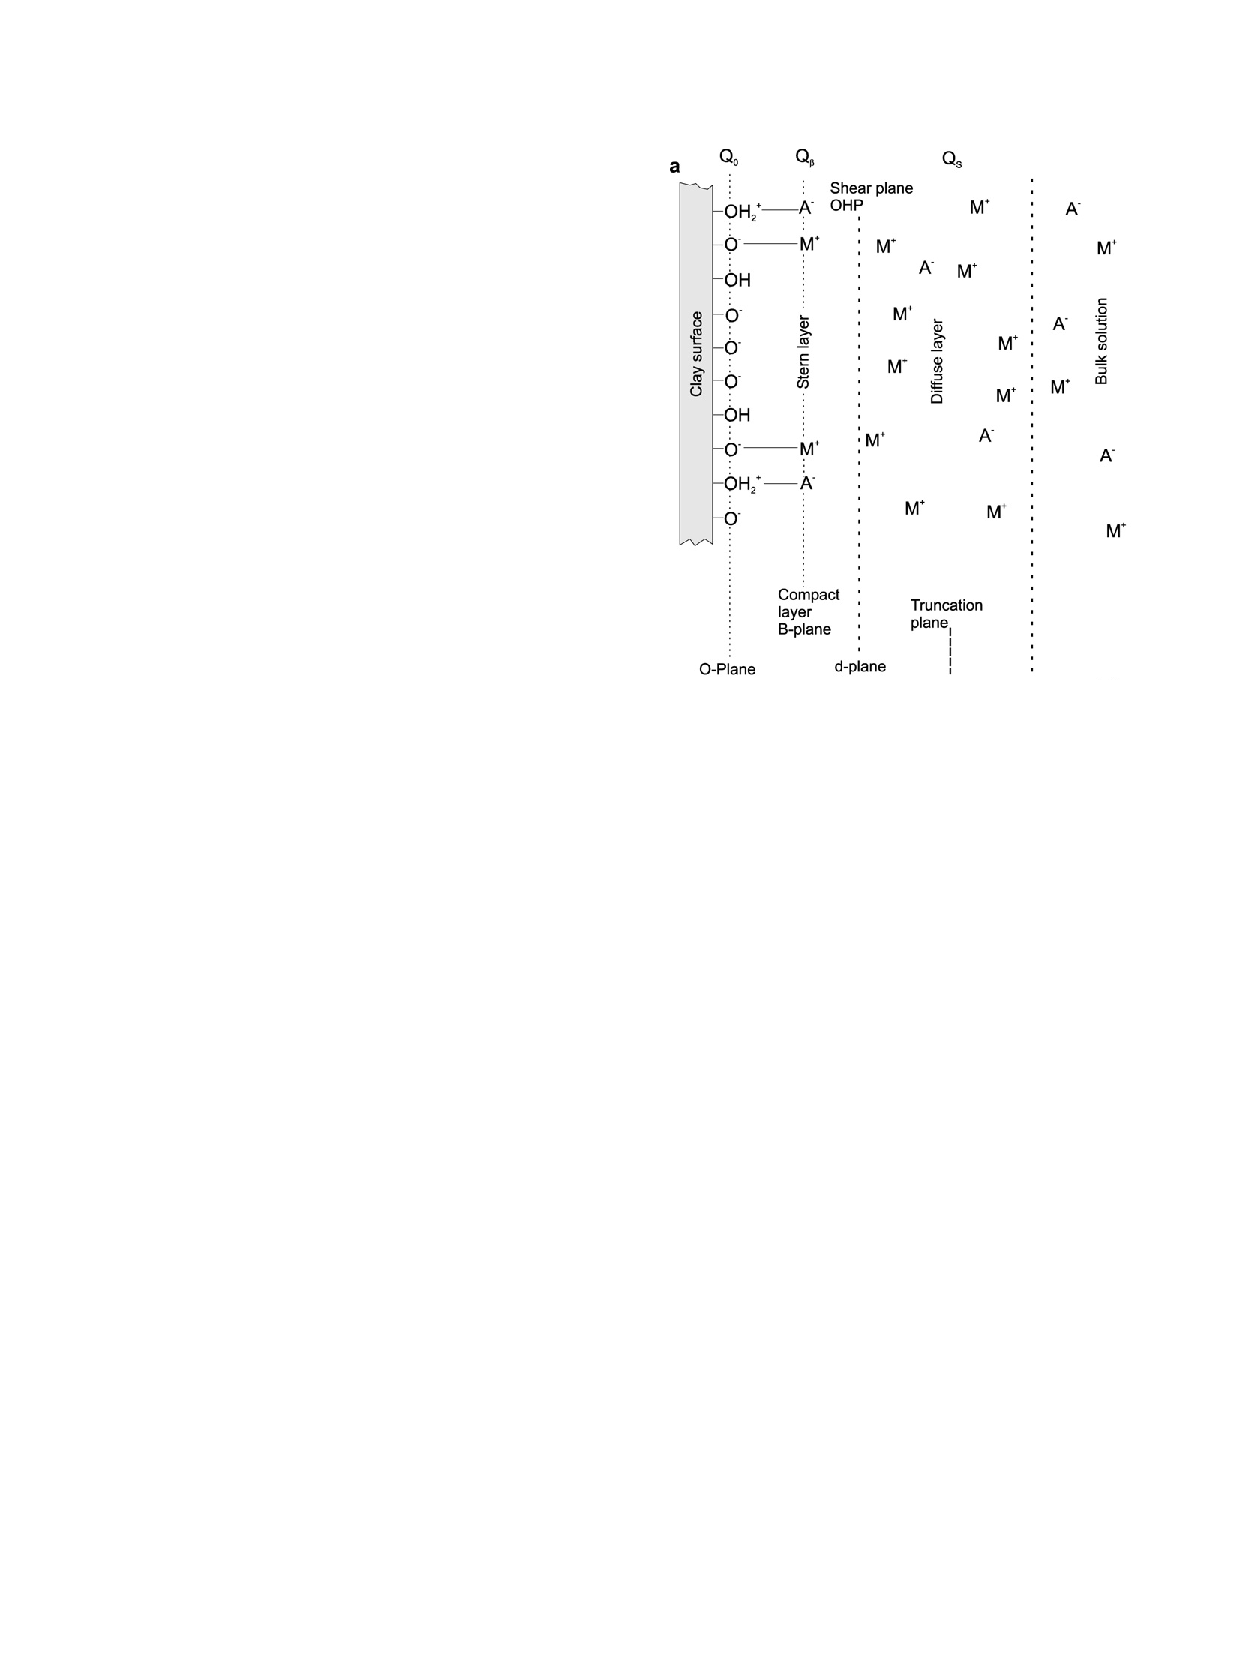
\includegraphics[width=0.75\linewidth]
                    {figs/sorption/goncalves-2007-TLM-Fig-a.pdf}
    \\[24pt]
    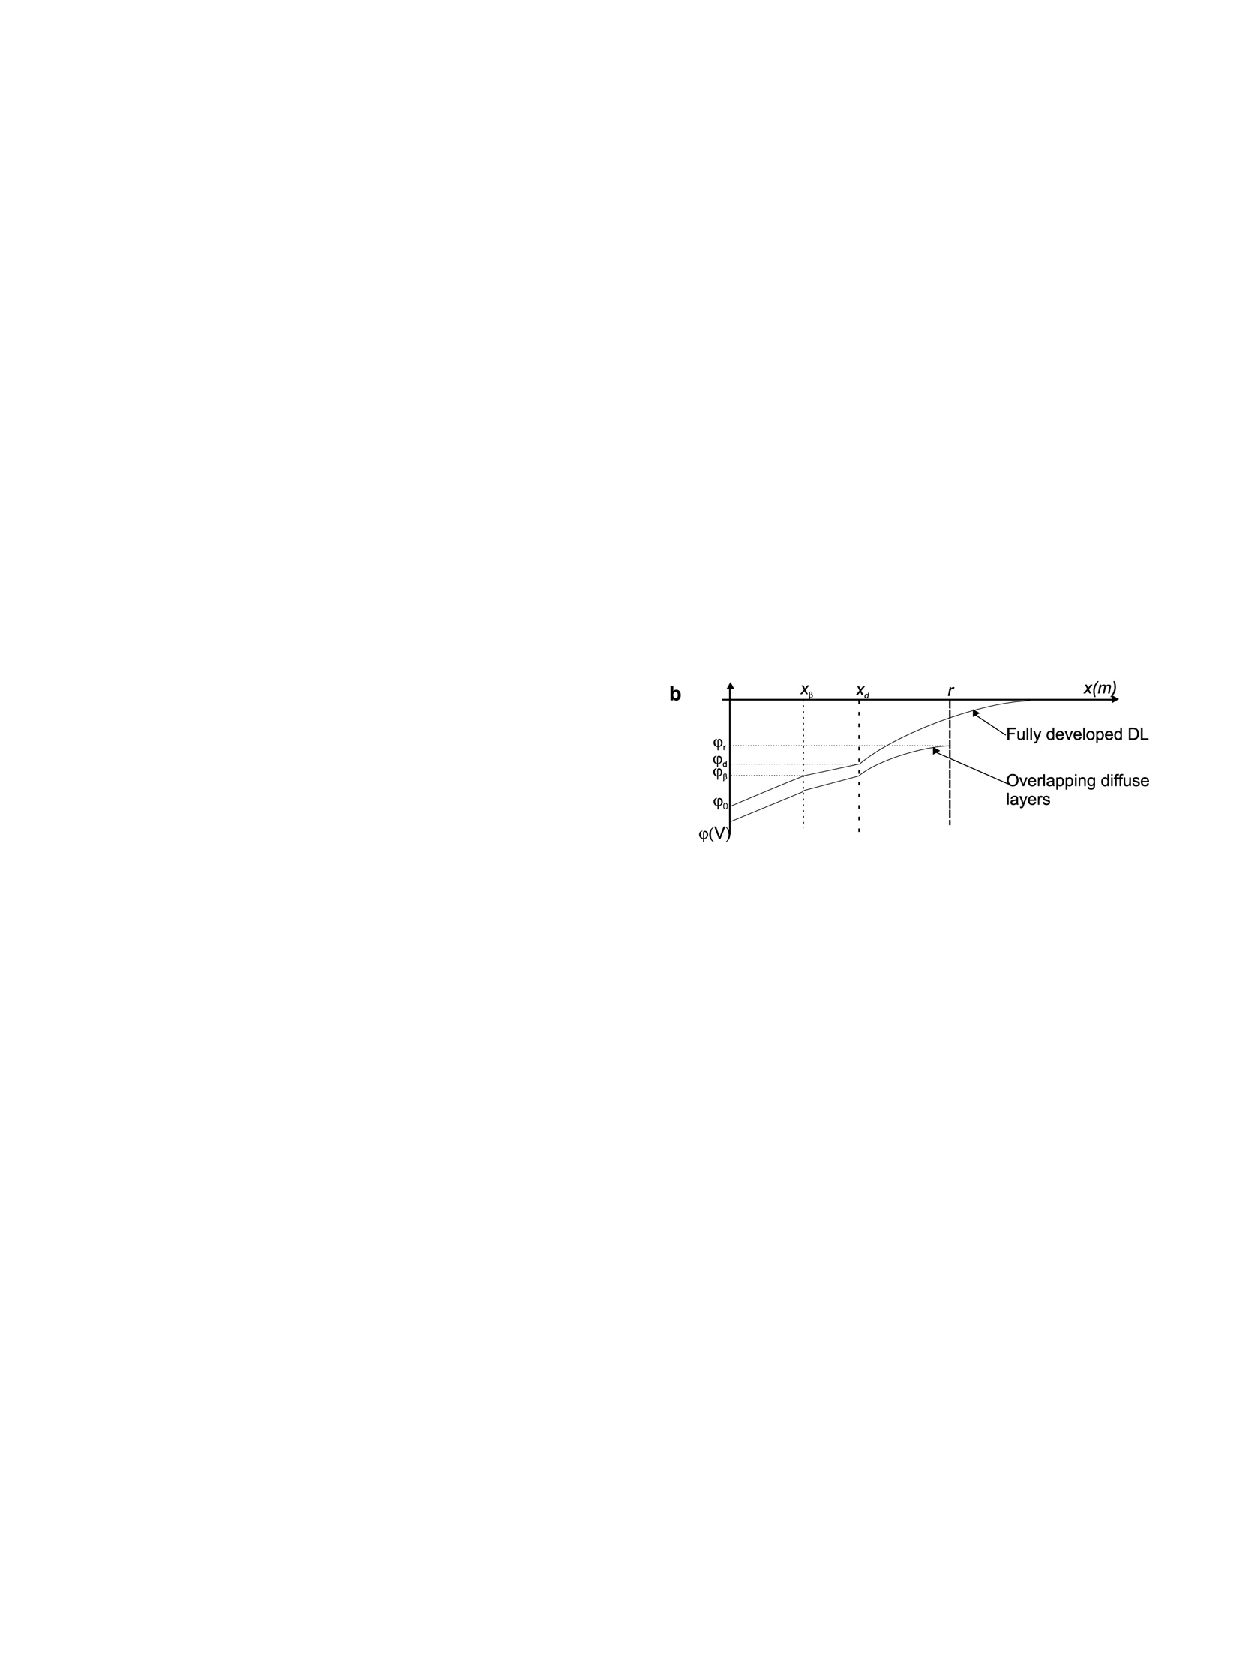
\includegraphics[width=0.75\linewidth]
                    {figs/sorption/goncalves-2007-TLM-Fig-b.pdf}
  \end{center} 
  \caption{Schematic of the TLM model from \citet{goncalves-2007}.}    
  \label{fig:triple-layer-model}
\end{figure}

\end{enumerate}
%  End electrostatic models

\end{enumerate}
%  End sub-models

\subsubsection{Common Data Needs for Sorption Models}
%\todo{Need to gather more requirements for this}

All sorption models will require access to a database of parameter values that are potentially independent of the specific contaminated site under consideration.  For example, the cation exchange capacity (CEC) of a mineral like smectite or kaolinite can be described with a range of values.  However, it is likely that site-specific experimental data will have to
be collected and either collected in a site-specific database, or serve as the basis of a site-specific lookup table.

%\todo{Davis: A database for Freundlich parameters is required? Is
% there such a database? In general, I think the model requirements
% for Kd, Langmuir, Freundlich, surface complexation and ion exchange
%  should state that it is likeley that experimental data have to be
%  collected with site-specific samples.}



%Spycher, Steefel

\subsection{Mineral Precipitation and Dissolution} 
\label{sec:mineralPrecipDissolution}

\subsubsection{Overview} 

Mineral precipitation and dissolution are among the most important
processes affecting the transport of contaminants in the subsurface.
They represent a class of heterogeneous reactions that require a
slightly different treatment than do reactions taking place within the
same phase.  Perhaps most importantly, a kinetic treatment of mineral
reactions requires the inclusion of the interfacial area between the
phases (water and mineral), or reactive surface area (see
Section~\ref{sec:ReactiveSurfaceArea}).  The reactive minerals may be
considered as pure, in which case their treatment is simplified by the
fact that their activity is always equal to one, or they may be solid
solutions, in which case their activities have to be determined as in
any other solution.  Minerals may be assumed to be at equilibrium with
the aqueous solution, in which case they can be included in the total
concentration in a fashion similar to the way in which equilibrium
secondary species are (Equation~\eqref{eq:AqueousComplexation_GrindEQ__12}), 
or they may be treated kinetically.  In most cases, it appears to be sufficient to
treat the minerals kinetically, since the equilibrium condition can be
regained by using reaction rates that are sufficiently fast relative
to the time scales of interest \citep{steefel_1996}.  This approach
also offers the advantage that the minerals can potentially be removed
as direct unknowns in the solution procedure within any one nonlinear
iteration cycle and updated only at the end of the time step.

\subsubsection{Kinetic Mineral-Water Rate Laws}

%Following the notation presented in Section~\ref{sec:mathframework},
The mineral reactions take the form
%
\begin{equation} 
 \sum_j\nu_{jm} \A_{j\a} \arrows \M_m,
 \label{heterogeneous-restated}
\end{equation}
%
for mineral $\M_m$ with reaction rate $I_{m\a}$ and stoichiometric
coefficients $\nu_{jm}$.  The sum of the mineral reaction rates
affecting component $j$ in phase $\a$ can be written as
%
\begin{equation} 
 R_{j\a} \eq \sum_m\nu_{jm} I_{m{\a}}.
 \label{eq:MineralReactionSummation}
\end{equation} 
In most cases, this will involve water as the fluid phase.
Equation~\eqref{eq:MineralReactionSummation} implies that component $j$
may be involved in any number of parallel mineral reaction pathways
(even within the same phase), with each potentially described by its
own rate law.  Changes in mineral concentrations are described by the
equation
%
\begin{equation}
  \frac{\partial \phi_m}{\partial t} \eq \overline V_m \sum_\a I_{m\a},
\end{equation} 
%
with molar volume $\overline V_m$ and where the sum over $\a$ on the
right-hand side is over all fluid phases that react with the $m$th
mineral.

We use a kinetic rate law based on the assumption that attachment and detachment of ions from mineral surfaces is the rate--limiting step (i.e., a surface reaction-controlled rate law). It does not mean, however, that one cannot obtain overall transport control on the mineral dissolution or precipitation rate since this depends on the magnitude of the reaction rate relative to the macroscopic transport rates. The rate laws used for mineral precipitation and dissolution are based loosely on transition state theory \citep{lasaga_1981,aagaard_1982,lasaga_1984}). 

\paragraph{TST Type Rate Law.}

This formulation gives the dependence of the rate on the saturation state of the solution with respect to a particular mineral as a function of the ion activity product, $Q_{s} $, defined by 
\begin{equation} \label{eq:Mineral3}  
  Q_{m} =\prod _{j=1}^{N_{c} } \, a_{j}^{\nu _{jm} } , 
\end{equation} 
where the $a_{j} $ are the activities of the primary species used in writing the dissolution reaction for the mineral and $\nu _{jm}$ are stoichiometric reaction coefficients. In order to incorporate the strong pH dependence of most mineral dissolution and precipitation reactions far from equilibrium, parallel rate laws are used which are summed to give the overall reaction rate law for a particular mineral in phase $\a$
\begin{equation} \label{eq:Mineral4} 
  I_{m\a} =-A_{m\a} \left\{ \sum _{l=1}^{N_{rm} } \, k_{l} 
  \left(\prod _{i=1}^{N_{c} +N_{x} } \, a_{i}^{p_{il} } \right) 
  \mathop{\left[1-\mathop{\left(\frac{Q_{m} }{K_{m} } \right)}
  \nolimits^{M_l} \right]}\nolimits^{n_l} \right\} , 
\end{equation} 
where $k_{l} $ is the far from equilibrium dissolution rate constant for the $l$th parallel reaction, $p_{il}$ is the exponential dependence on species $i$ of the $l$th parallel reaction (i.e., the reaction order), $K_{m} $ is the equilibrium constant, $N_{rm}$ is the number of parallel reactions within phase $\a$, and $A_{m\a} $ refers to the surface area of the reacting mineral in contact with phase $\a$ (m$^2$ mineral m$^{-3}$ porous medium). The exponents $n_l$ and $M_l$ allow for nonlinear dependencies on the affinity term and are normally taken from experimental studies. The term $\prod _{i=1}^{N_{c} +N_{x} } \, a_{i}^{p_{il}} $ incorporates the effects of various ions in solution on the far from equilibrium dissolution rate. This is most commonly the solution pH or hydroxyl ion activity but may include other electrolytes as well.

The temperature dependence of the reaction rate constant can be expressed reasonably well via an Arrhenius equation \citep{lasaga_1984}. Since many rate constants are reported at 25$^{\circ } $C, it is more convenient to write the rate constant at some temperature as 
\begin{equation} \label{eq:Mineral5} 
  k=k_{25} \; \rm{exp} \left[ \frac{-E_{a} }{R} \left( \frac{1}{T} -\frac{1}{298.15} \right) \right], 
\end{equation} 
where $E_{a} $ is the activation energy, $k_{25} $ is the rate constant at 25$^{\circ } $C, $R$ is the gas constant, and $T$ is temperature in the Kelvin scale. 

\paragraph{Nonlinear Parallel Mineral Rate Laws.}

The rate law proposed by \citet{hellmann2006dissolution}, based on experimental data for albite, can be used for dissolution of silicate minerals. One rate law describes far from equilibrium dissolution behavior with a rate constant $k_2$, and one rate law describes close to equilibrium behavior ($k_1$):
\begin{equation}  \label{eq:Mineral6} 
  I_{m\a_\circ} \eq A_{m\a_\circ}  \{ k_{1} [1-\exp (-m_{1} g^{m_{2} } )]+k_{2} [1-\exp (-g)]^{m_{3} }  \},
\end{equation}                
where $g$ represents $\frac{|\Delta G_r|}{RT}$ and the fitted parameters $m_1$, $m_2$ and $m_3$ have values of $7.98 \times 10^{-5}$, $3.81$ and $1.17$ \citep{hellmann2006dissolution}. Here again the assumption is that the phase in question, $\a_\circ$, is water.  This formulation is consistent with theoretical and experimental considerations which suggest that far-from-equilibrium dissolution is characterized by the opening of etch pits and rapid propagation of step waves, whereas close-to-equilibrium dissolution in the absence of etch pits is localized to surface defects. 

\paragraph{Dissolution Only.}

The simplest form of a dissolution only rate law would be a completely irreversible reaction with no back reaction (i.e., no precipitation).  However, it may be desirable to have a rate law which slows as equilibrium is approached, even though the back reaction cannot really be demonstrated.  Such a rate law is likely applicable to the dissolution of albite at low temperature, since dissolution can be demonstrated while precipitation cannot.  There is clear evidence in the case of plagioclase that the rate of dissolution does slow, so it is important to be able to include this in the code \citep{maher2009role}.  Similarly, it was found that kaolinite could not be described with a single rate law that was continuous for both dissolution and precipitation \citep{yang2008kaolinite}.  To describe both precipitation and dissolution of kaolinite, therefore, one can use distinct dissolution-only and precipitation-only rate laws.

A rate law for dissolution only could in principle include any number of rate laws
having a TST (linear or nonlinear) form, but with the added code (here presented as a linear TST rate with no dependence on dissolved or sorbed species far from equilibrium for the sake of simplicity):
\begin{eqnarray}
I_{m\a_\circ} \eq
  \begin{cases}
   -A_{m\a_\circ} \mathop{\left[1-\mathop{\left(\frac{Q_{m} }{K_{m} } \right)} \right]} & \text{if $I_{m\a_\circ} < 0$},\\
   0 & \text{if $I_{m\a_\circ} > 0$}.
  \end{cases}
\end{eqnarray}
%\[
 % r_{s} = \left\{ 
%\begin{array}{l l}
%  =-A_{s} \mathop{\left[1-\mathop{\left(\frac{Q_{s} }{K_{s} } \right)} \right]} & \quad \mbox{if $r_{S}<0$}\\
%  =  0 & \quad \mbox{if $r_{S}>0$}\\ \end{array} \right. \]  \label{dissolutiononly}

%Could have the following
%\subparagraph{Assumptions}
%\subparagraph{Data Needs}

\paragraph{Precipitation Only.}

A precipitation-only rate law takes a similar form to that of dissolution-only
\begin{eqnarray}
I_{m\a_\circ} \eq
  \begin{cases}
   A_{m\a_\circ} \mathop{\left[1-\mathop{\left(\frac{Q_{m} }{K_{m} } \right)} \right]} & \text{if $I_{m\a_\circ} > 0$},\\
   0 & \text{if $I_{m\a_\circ} < 0$}.
  \end{cases}
\end{eqnarray}

%Could have the following
\subsubsection{Assumptions and Applicability for Rate Laws}

All of the rate laws described above use reactive surface area as an important parameter (see Section~\ref{sec:ReactiveSurfaceArea}).  This is because most of the rates determined for mineral dissolution and precipitation are based on normalization to physical surface area.  Rate laws that consider the actual kind and density of reactive sites are possible, but so far are difficult to implement at the field scale.

\subsubsection{Data Needs for Rate Laws}

Data needs for mineral dissolution and precipitation are considerable and help to explain why these processes have not always been included in subsurface environmental management codes.  In the case of mineral dissolution, it is necessary to know the reactive surface area of the dissolving mineral in contact with the mobile fluid phase.  Reactive surface area within immobile zones may contribute to the reactivity as well over long time scales via diffusion, so normally must be considered as well (see Section~\ref{sec:ReactiveSurfaceArea}).  

Reactive surface area is an even more difficult topic in the case of mineral precipitation.  Here seeds may be created by nucleation, the seeds may growth via crystal growth and/or ripening and agglomeration \citep{steefel1990new}.  Some proposed methods for including the evolution of reactive surface area are given in Section~\ref{sec:ReactiveSurfaceArea}.  
%Could have the following
%\subparagraph{Assumptions}
%\subparagraph{Data Needs}

%Steefel
%\paragraph{Nucleation.}

%Could have the following
%\subparagraph{Assumptions}
%\subparagraph{Data Needs}

%\paragraph{Solid Solutions.}

%Could have the following
%\subparagraph{Assumptions}
%\subparagraph{Data Needs}

%\subsubsection{Common Data Needs for Mineral Precipitation/Dissolution Models}

\subsubsection{Reactive Surface Area Evolution}  
\label{sec:ReactiveSurfaceArea}

Surface area is a key parameter affecting mineral dissolution and
precipitation rates, as well as the extent of aqueous species (e.g.,
contaminants) sorption onto mineral surfaces.  Accordingly, surface
area is one of the variables that appear in mineral dissolution and
precipitation rate laws, Section~\ref{sec:mineralPrecipDissolution},
as well as in expressions needed to compute sorption site
concentration for surface complexation models,
Section~\ref{sec:surfaceComplexation}.  The incorporation and
treatment of surface areas into reactive transport simulations can be
broken down into two parts: initial surface areas,
Equation~\eqref{eq:RSA:1}, which can be either directly input into the
model if known, or estimated from input geometric data and
Equation~\eqref{eq:FractureSurfaceArea} the actual evolution of surface areas
(starting from input or calculated initial values) upon mineral
dissolution or precipitation.

Initial surface areas can be estimated from laboratory measurements
for pure minerals or bulk sediments.  However, actual ``reactive''
surface areas in natural systems are largely unknown, and have been
shown to be typically smaller than laboratory measurements by several
orders of magnitude, and in much closer agreement with geometric
mineral surface areas.  For this reason, it is not uncommon to
estimate initial reactive surface areas from available geometric data
on the size and shape of mineral grains in porous media, or from data
on fracture coverage (thus spacing) in fractured rocks.  This can be
achieved either internally or externally prior to input, using
relatively simple mathematical expressions that do not require a high
level of accuracy given the large variability of this parameter in
natural systems.  Alternatively, initial surface areas can be
calibrated during the course of reactive transport simulations.

Once initial (reactive) surface areas have been determined, the
evolution of these areas upon mineral reaction needs to be captured in
a manner that is consistent with field and experimental observations.
For dissolving minerals in water-saturated systems, the evolution of
reactive surface area can be calculated, as a first approximation, by
assuming some proportionality between the amount of mineral present
and its surface area.  In such case, simple relationships can be
developed relating surface area with mineral volume fraction, as shown
further below.  In unsaturated systems, however, the problem is
complicated by the fact that reactive surface areas are not only
function of mineral volume fractions, but also potentially of liquid
saturation.  While water serves as the wetting phase in most cases,
and thus in in contact with the solid grains in the medium, at low
saturations the coverage may become discontinuous.  In this case, as a
first approximation, the reactive surface area in contact with the
phase (in the case of water, the "wetting phase") can be assumed to be
proportional to liquid saturation.

Predicting the evolution of surface area from the onset of, and
during, mineral precipitation is less straightforward.  If a mineral
forms on existing surfaces (of the same mineral and/or on surfaces of
existing precursors), the surface area can be assumed to evolve with
some proportionality to the current volume fraction of the mineral (or
precursor mineral(s)).  However, if a mineral actually nucleates from
solution, without precursors, a rigorous treatment of nucleation is
required \citep{steefel1990new}.  Such rigorous treatment, however, is
deemed outside the scope of current model requirements, primarily
because input parameters for nucleation models are scarce for most
minerals.  Instead, an approximate treatment can be considered,
yielding a trend of surface area evolution similar to that expected
upon nucleation (i.e., initially large surface areas upon nucleation
decreasing with growth).  This general behavior can be captured by
assuming that the initial (first formed, minimum) amount and grain
size of a nucleating mineral is known.  Using these two (input)
parameters (i.e., minimum/initial volume fraction and grain size), the
initial number of precipitating mineral grains and their surface area
can be easily computed for each mineral assuming simple grain
geometries (e.g., spheres).  Upon further precipitation, the evolution
of surface area can then be computed as a function of mineral grain
size, with mineral grains growing with some proportionality to the
amount of mineral precipitation.  As such, surface areas initially
decrease with increasing mineral amounts, starting from initially
large values at small initial grain sizes.  For each mineral, this
decrease in surface area with growth can be assumed to continue until
the surface area reaches some preset (input) value corresponding to
the surface area of the ``bulk'' mineral.  At this point, the surface
area is assumed to evolve again with some direct proportionality to
volume fraction, as in the case of dissolving minerals.

The general methodology and formulation of the above-described
approach are presented further below.  Note that because surface areas
evolve relatively slowly in most systems, compared to other parameters
such as aqueous concentrations, surface areas can be computed
explicitly.  That is, surface areas computed at the end of a
flow/transport/reaction time step can be used as values for computing
reactive transport at the next time step.

\paragraph{Reactive Surface Area.}

The following general relationship can be used to compute reactive
surface areas of minerals as a function of time:
%
\begin{equation}
  A_{m\a} \eq \gamma_{m} \; \left( \phi_{m} A _{SS_m} \; 1000 \;
    \rho_{m} + \overline{A}_{m\a} \right),
 \label{eq:RSA:1}
\end{equation}
%
where $A_{m\a}$ is the effective reactive surface area of minerals
(m$^2$ mineral per m$^{-3}$ porous medium), $\gamma_{m}$ is the
fraction of the mineral's surface area that is in contact with the
phase (normally water), $\phi_m$ is the volume fraction of the
mineral, $A _{SS_m}$ is the specific surface area of the mineral
(m$^2$/g), $\rho_M$ is the dry density of the mineral (kg m$^{-3}$),
and the factor of 1000 converts from kg to g.  $\overline{A}_{m\a}$ is
the precursor surface area (m$^2$ mineral m$^{-3}$ medium).  The
fraction of the mineral surface area, $\gamma_{m}$, in contact with
the phase $\a$ may be estimated from petrographic observations, fitted
from field data, or potentially estimated based on as yet unspecified
relationship with phase (liquid) saturation.

An alternative expression for computing reactive surface area is given
by \citet{steefel-1994}
%
\begin{equation}  
  A_{m\a} \eq \gamma_{m}   A_{m\a}^{\circ}   
   \left(\frac{\phi_m}{\phi_{m}^{\circ} } \right),
 \label{eq:BulkSurfaceArea}
\end{equation} 
%
where $A_{m\a}^{\circ}$ and $\phi_{m}^{\circ}$ are the initial surface
area and volume fraction of the mineral, respectively.

In the case of secondary minerals that are not initially present and
where no precursor mineral occurs with a non-zero volume fraction,
both Eqns. \eqref{eq:RSA:1} and \eqref{eq:BulkSurfaceArea} can be modified
to include a ``threshold'' mineral volume fraction that is used just
for the purposes of calculating reactive surface area.  This mineral
mass is considered to be derived from a short-lived nucleation event
that quickly creates surface area upon which subsequent mineral growth
can occur.  The threshold volume fraction, $\phi_{nucl}$, can be
incorporated in the following way:
%
\begin{eqnarray}
  A_{m\a} \eq
 \begin{cases}
   \gamma_{m} \; \left( \phi_{m} A _{SS_m} \; 1000 \; \rho_{m} \right)    & 
   \text{if $\phi_{m}  > \phi_{m}^{nucl}$},\\
   \gamma_{m} \; \left( \phi_{nucl} A _{SS_m} \; 1000 \; \rho_{m} \right)    & 
   \text{if $\phi_{m}  < \phi_{m}^{nucl}$}.\\
 \end{cases}
\end{eqnarray}
%
Such a procedure obviates the need for a more complicated formulation
such as that found in \citet{steefel1990new}.

Another option to be implemented involves a simple geometric method
for calculating surface area \citep{lasaga_1984}. If a simple cubic
packing of spherical grains of radius $r$, is considered, then the
cubic arrangement of spheres yields, in a cube of side $4r$ and volume
$(4r)^3$, a total of 8 spheres, each of radius $r$, volume 
$\frac{4\pi r^3}{3}$, and area $4\pi r^2$.  Thus the surface area 
$A_{nucl}$ (as the area of the spheres divided by the volume of the
cube) can be computed as
%
\begin{equation}
  A_{m\a} \eq \gamma_{m} \frac{0.5}{r} ,         
  \label{eq:RSA:5}
\end{equation} 
%
where $r$ is the average grain size of the mineral.  A more
comprehensive approach involving crystal size distributions has been
proposed by \citet{steefel1990new}.

\paragraph{Estimation of Reactive Surface Areas for Fractures.}
%
In a dual permeability (fracture-matrix) system, the surface area of
the fracture in contact with the mobile fluid phase, $A_F$ (in units
of m$^2$ fracture m$^{-3}$ medium) is \citep{steefel-1994}
%
\begin{equation}
  A_F \eq \varphi_{F} \frac{2}{\delta},
 \label{eq:FractureSurfaceArea} 
\end{equation}
where $\varphi_{F}$ is the fracture porosity and $\delta$ is the
fracture aperture.  To calculate the amount of mineral surface area
present along the fracture, one can use the volume fraction of the
primary dissolving phase as an estimate of the fraction of the
fracture surface made up of that mineral
%
\begin{equation}
 A_{m\a} \eq \varphi_{F} \phi_{m} \frac{2}{\delta}.
 \label{eq:MineralSurfaceArea}
\end{equation}
For precipitation, various schemes are possible.  If the assumption is
made that mineral precipitation can occur anywhere along the fracture
surface, then \eqref{eq:FractureSurfaceArea} 
%
%\todo{Carl check this equation reference, I fixed a duplicate label
%  -JDM}
%
can be used without modification.  For partially wetted fractures, a correction can be 
introduced to reduce the reactive surface area:
%
\begin{equation} 
  A_{m\a} \eq \varphi_{F} \gamma_m \phi_{m} \frac{2}{\delta},
  \label{eq:WettedFractureSurfaceArea}
\end{equation}
%
where $\gamma_m$ is the fraction of the fracture actually in contact
with the reactive phase (normally water).
















